\cfoot{\page\textbackslash of \pageref{lastpage}} %Skal vise x antal sider af y
\chapter{Udviklingsmetoder}
For at få et bedre overblik over, hvilken metode der vil være bedst til at styre driften for et MMO, er det relevant at kigge på forskellige udviklingsmetoder. I følgende afsnit, vil der blive kigget nærmere på metoderne; Vandfaldsmodellen, SCRUM og Unified Process(UP). Hvert afsnit vil indeholde en kort beskrivelse, samt nogle af de fordele og ulemper der er ved at bruge metoden.\\

\section{Vandfaldsmodellen}
%Vandfaldsmodellen er en iterativ udviklingsmetode, der er simpel og let anvendelig.\cite{Waterfall} 
%Navnet udspringer af den måde, som metoden gennemgår sine seks faser på, som kan ses i figur ? nedenfor. Essensen ved vandfaldsmodellen er, at man først kan fortsætte til næste fase i udviklingen, når den fase man er i er helt færdig.
Det er vigtigt her, at bemærke i figur ?, at der først testes efter udviklingen i projektet. 
Dette har for eksempel den konsekvens, at projektet er færdiglavet, men ikke er blevet testet igennem, for eventuelle fejl og mangler, og denne udviklingsmetode gør ikke brug af at springe tilbage i faserne, når de først er blevet lavet. 
Det vil sige, at når konstruktionsfasen er færdig, kan man ikke gå tilbage og ændre i den, uanset hvad for eksempel resultatet af testfasen viser. 
Denne metode er oftest brugt ved kortere projekter, hvor kravene er meget specifikke og der er så få parametre udefra som muligt, der kan gå ind og ændre ved projektet.\\
%\\
%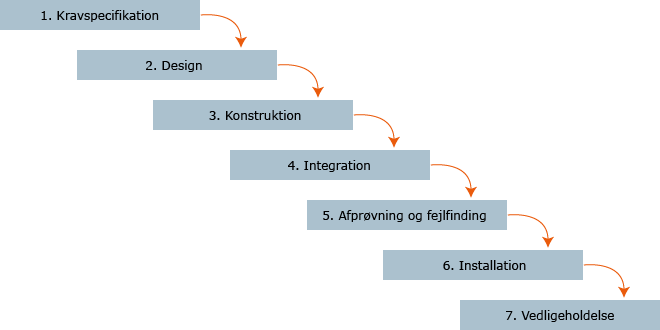
\includegraphics[scale=0.1]{figures/Vandfaldsmodellen}
%\\
\section{Anden sektion}

\subsection{under sektion}
